\documentclass[hidelinks, 12pt, twocolumn]{article}
\usepackage{graphicx}
\usepackage{lipsum}
\usepackage{hyperref}
\usepackage{xcolor}
\usepackage{amsmath, amssymb}
\usepackage{cuted}
\usepackage{amsbsy}
\setlength{\columnsep}{1cm}
\usepackage[margin=0.7in]{geometry}
\usepackage[style=numeric-comp,useprefix,hyperref,backend=bibtex]{biblatex}
\graphicspath{{../img/}}
\usepackage{endnotes}
\usepackage{float}
\title{Wine Project Report}
\author{Nocera Ruggero (S292442) \\ Quarta Matteo (S292477)}
\date{}


\begin{document}

\maketitle
\begin{strip}
    {\bf Abstract}
    In this report we analyze how effective are different classifiers and different preprocessing techniques applied to a binary classification task.
    The dataset used to train and test the models taken in consideration is a modified version of
    the one provided by {\it Modeling wine preferences by data mining from physicochemical properties}
    from {\it Decision Support Systems, Elsevier} (P. Cortez, A. Cerdeira, F. Almeida, T. Matos and J. Reis.).
    Due to limited time and computational power, results may be just close-to or far-from optimal, depending on the time required to train a model.
    Although reasonable results have been obtained, the purpose of this report is not to describe the best possible application,
    but to make an analysis of the various techniques presented during the course.

\end{strip}
\tableofcontents


\section{Preliminary Data Analysis}
\subsection{Feature Distribution}

Before discussing the models, their implementation and their effectiveness we briefly take a look at how the features are distributed.
For convenience we shall now report the legend just once, but keep in mind that in the following pictures the red color is associated to class 0 
(which we will also be referring to as class {\it Bad}) and the green color is associated to class 1 (which will be class {\it Good}).

\begin{figure}[H] 
    \caption{Histogram of Class' Features}
    \label{fig:disthist}
    {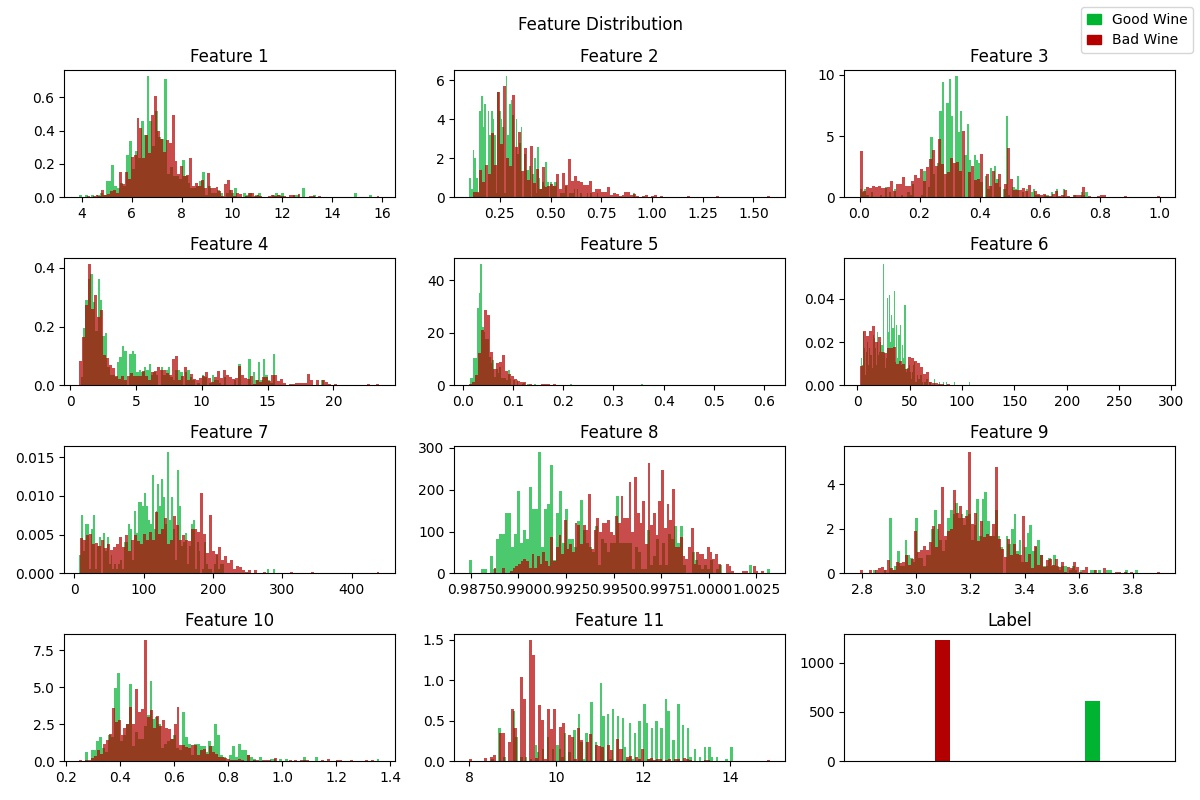
\includegraphics[width=\linewidth]{dist.jpg}}
\end{figure}

First of all, our training dataset is unbalanced. 
In the next pages we will be classifying samples obtained from a K-Fold\footnotemark Validation approach, using a theoretical threshold given by:

$$ t = -\log{\frac{\pi}{1-\pi}} $$

For the threshold to be optimal, we should use the empirical prior $\pi \approx 0.33$ based on a frequentist approach;
Instead we will be using a non-optimal prior $\tilde{\pi} = .5$ as it is the application we are going to be targeting
.
\footnotetext{More on the value of K later}

We can notice some things:
while some features are similar between class Good and class Bad (e.g. Feature 1) others differ substantially 
and could be helpful in discriminating samples (e.g. Feature 8).

The features are also distributed in different ways: 
some do look Gaussian distributed (e.g. Feature 9) or regular enough
(e.g. Feature 5) and could thus be well estimated by Gaussian models\footnotemark 
, other act in a more irregular way.

\footnotetext{Both Gaussian Classifiers and GMMs}.

To take a closer look we project the data on the two dimensional plane. 
We will be using 3 methods: PCA\footnotemark , Normalization + PCA, Normalization + Whitening.

\footnotetext{No data centering applied before}

\begin{figure}[H]     
    {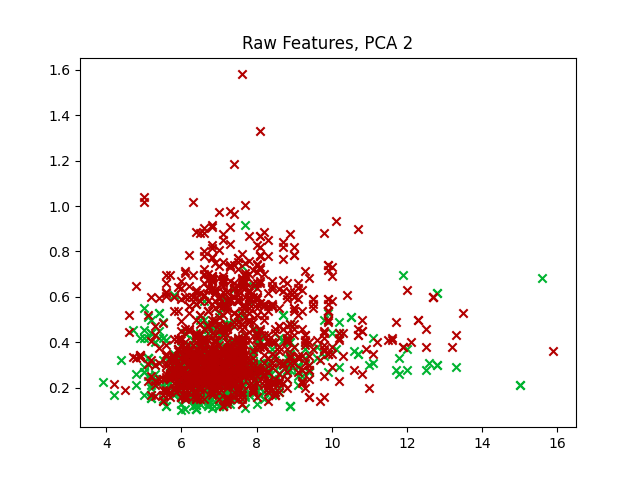
\includegraphics[width=\linewidth]{2DRAW.png}}
    \caption{2D-PCA Projection}
    \label{fig:2DRAW}
\end{figure}

The points don't seem much correlated, we expect Whitening to not be of much use.

\begin{figure}[H] 
    {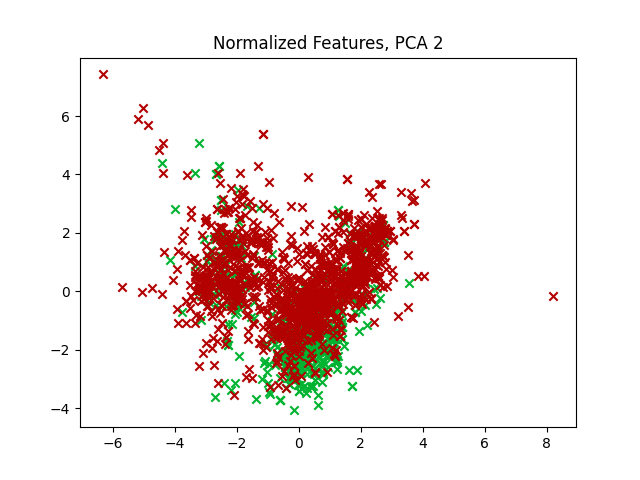
\includegraphics[width=\linewidth]{2DNorm.png}}
    \caption{2D-PCA Projection, Normalized Data}
    \label{fig:2DNORM}
\end{figure}

The normalized projection splits data in two clusters, 
each containing some samples of each class, 
but some points of different class also do get apart one another:
normalization could be of use

Our chosen normalization technique is Z-Normalization.
From a preliminary, off-record analysis we found Gaussianization to produce
similar results while being slower.

Lastly, the Whitened data.

\begin{figure}[H] 
    {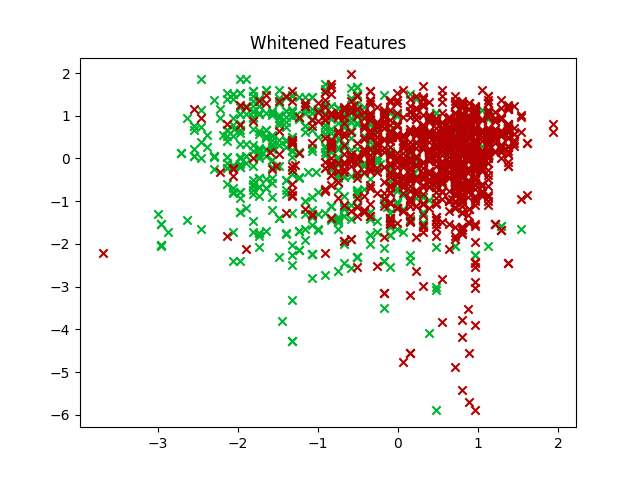
\includegraphics[width=\linewidth]{2DWhitened.png}}
    \label{fig:2DWHI}
    \caption{2D-PCA Projection, Whitened Data}
\end{figure}

Results are more interesting than expected,
doing well in getting points of different class
apart one another.

\section{Pre-Processing Analysis}

In this section we will run the models without trying to optimize them as much as we can.

\subsection{Pre-Processing MVG Classifiers}

Since MVG classifiers are fairly similar, 
we will discard the less promising ones now.

\begin{table}[H] 
    \centering
    \begin{tabular}{||c|c|c|c||}
        \hline
        Type & PCA & DCF & minDCF \\
        \hline
        \hline
        Raw   & 8  & 0.375 & {\bf 0.321} \\
        Raw   & 9  & {\bf 0.360} & 0.326 \\
        Norm. & 10 & 0.419 & 0.330 \\
        Norm. & 11 & 0.424 & 0.322 \\
        Whit. & 11 & 0.424 & 0.322 \\
        Whit. & 8  & 0.392 & 0.342 \\
        \hline
    \end{tabular}
    \caption{Full-Covariance MVG - Best Results}
    \label{fullcovtab}
\end{table}

    
\begin{table}[H] 
    \centering
    \begin{tabular}{||c|c|c|c||}
        \hline
        Type & PCA & DCF & minDCF \\
        \hline
        \hline
        Raw   & 11 & {\bf 0.342} & 0.332 \\
        Norm. & {\bf 5}  & 0.414 & {\bf 0.330} \\
        Norm. & 11 & {\bf 0.342} & 0.332 \\
        Whit. & 11 & {\bf 0.342} & 0.332 \\
        \hline
    \end{tabular}
    \caption{Tied-Covariance MVG - Best Results}
    \label{tiedcovtab}
\end{table}

\begin{table}[H]
    \centering
        \begin{tabular}{||c|c|c|c||}
            \hline
            Type & PCA & DCF & minDCF \\
            \hline
            \hline
            Raw   & 9  & 0.404 &  0.365 \\
            Raw   & 7  & {\bf 0.391} &  0.370 \\
            Norm. & 9  & 0.428 &  0.350 \\
            Whit. & 11 & 0.460 &  {\bf 0.344} \\
            Whit. & 5  & 0.394 &  0.374 \\
            \hline
    \end{tabular}
    \caption{Naive-Bayes MVG - Best Results}
    \label{naivetab}
\end{table}

The results are in line with our assumptions.
Looking again at picture \ref{fig:2DRAW} we wouldn't expect the Naive Bayes to perform much differently from the Full Covariance one.
The best model, with a modest margin, is the Tied Covariance one so
this will be our chosen one.

Notice that while the Tied Covaraiance model achieved the best DCF\footnotemark of all classifiers,
the MVG achieved the lowest Minimum DCF values, hiting that it may be the model
wit the best theoretical separation capabilities.
\footnotetext{Normalized DCF, $\pi_T = .5$, equal costs}

Whitening as expected is of no use, we won't further experiment it.

\subsection{Pre-Processing for GMMs}

For the GMM model we arbitrairly train it with four components.
Optimizations will be made later.

The starting point for our EM algorithm is identity covariance matrices and means placed around the dataset mean.

\begin{table}[H]
    \centering
        \begin{tabular}{||c|c|c|c||}
            \hline
            Type & PCA & DCF & minDCF \\
            \hline
            \hline
            Raw & No & 0.410 & {\bf 0.394}  \\
            Normalized &  9 & {\bf 0.407} & 0.402 \\
            Whitened & 4 & 0.429 & 0.420 \\
            \hline
    \end{tabular}
    \caption{GMM - Best Results}
    \label{tab:gmmresults}
\end{table}

As for our Gaussian Classifiers, whitening is not useful, but we will further experiment with normalization.
High dimensionality seems preferred.

\subsection{Pre-Processing for SVMs}

Differently for what we did up to now, given the non-probabilistic nature of SVM scores,
we will be deciding our optimal model for both types of kernel SVMs on just minimum DCFs values.

\subsubsection{Pre-Processing for Linear SVM}

\begin{table}[H]
    \centering
        \begin{tabular}{||c|c|c|c|c|c||}
            \hline
            Type & K & C & PCA  & minDCF \\
            \hline
            \hline
            Raw & 0 & 10.0 & 6 & 0.568  \\
            Norm. & 10 & 0.1 & 9 &  {\bf 0.330}  \\
            Whit. & 1.0 & 1.0 & 9 &  0.331  \\
            \hline
    \end{tabular}
    \caption{Linear SVM - Best Results}
\end{table}

The Linear SVM model performed much better with normalization.
Whitening looks again irrelevant.

PCA is useful to obtain lower values of minimum DCF in all cases, even if the model trained
with raw features performs worse than models trained with preprocessed features.

\subsubsection{Pre-Processing for Polynomial Kernel SVMs}

The dummy parameters chosen for execution are:

$$k({\bf x_1}, {\bf x_2}) = ({\bf x}_1^T{\bf x}_2+1)^2+0.5 $$

\begin{table}[H]
    \centering
        \begin{tabular}{||c|c|c|c||}
            \hline
            Type & PCA & minDCF \\
            \hline
            \hline
            Raw & 7 & 0.545  \\
            Normalized & 6 & {\bf 0.381}  \\
            Whitened & 11 & 0.393  \\
            \hline
        \end{tabular}
        \caption{Polynomail Kernel SVM - Best Results}
        \label{polypreprocessing}
\end{table}

Here we notice some differences with previous models:
normalization greatly improves our classification,
and small dimensionality obtain lower DCFs, 
even if not significanlty.

Again, whitening does not make any difference.

\subsection{Pre-Processing for RBF Kernel SVMs}

The dummy parameters for the RBF Kernel are:

$$\displaystyle k({\bf x_1}, {\bf x_2}) = e^{-\gamma||{\bf x}_1 - {\bf x}_2||^2} + b = e^{-0.05||{\bf x}_1 - {\bf x}_2||^2} + 0.05 $$

\begin{table}[H]
    \centering
        \begin{tabular}{||c|c|c||}
            \hline
            Type & PCA & minDCF \\
            \hline
            \hline
                Raw & 10 & 0.579 \\ 
                Normalized & No & {\bf 0.352} \\ 
                Whitened & No & {\bf 0.352} \\ 
            \hline
    \end{tabular}
    \caption{RBF Kernel SVM - Best Results}
\end{table}

Opposed to polynomial SVMs,
RBF prefers high dimensionality.
Also in this case normalization plays and important role while whitening does not look useful.

So far, this is our most promising model.

\subsection{Pre-Processing for Logistic Regression Model}

\subsubsection{Linear Logistic Regression}


Normalization helps in obtaining lower minimum DCFs compared to raw features,
and higher dimensionality is preferred.
Whitening in this case looks extremely harmful and we won't further analyze it.

\begin{table}[H]
    \centering
    \small
        \begin{tabular}{||c|c|c|c||}
            \hline
            Type & PCA & DCF & minDCF \\
            \hline
            \hline
            Raw ($\lambda = 0.0001$) & 10 & 0.369 &  0.342  \\
            Norm. ($\lambda = 0.01$) & 9 & 0.369 &  {\bf 0.336}  \\
            Whit. ($\lambda = 0.0001$) & No & 0.549 &  0.503  \\
            \hline
    \end{tabular}
    \caption{Linear Logistic Regression - Best Results}
\end{table}

The reported results are obtained through optimized parameters.

\subsubsection{Quadratic Logistic Regression}

In the Quadratic Logistic Regression, after the preprocessing stage, the features space
was expanded through 

$$ {\bf \boldsymbol{\phi}(x)} = {
    \begin{bmatrix}
    vec\langle{\bf xx^T}\rangle\\
    {\bf x}
    \end{bmatrix}}
$$ 

Whitening does not harm as in the linear case but it isn't helpful either, and we will again discard it.
PCA is more helpful when working with raw features.

\begin{table}[H]
    \centering
    \small
        \begin{tabular}{||c|c|c|c||}
            \hline
            Type & PCA & DCF & minDCF \\
            \hline
            \hline
            Raw ($\lambda = 0.1$) & 6 & 0.385 &  0.366  \\
            Norm. ($\lambda = 0.001$) & 10 & 0.324 &  {\bf 0.307}  \\
            Whit. ($\lambda = 0.001$) & 10 & 0.324 &  {\bf 0.307}  \\
            \hline
    \end{tabular}
    \caption{Quadratic Logistic Regression - Best Results}
\end{table}

\section{Optimizing Models}

\subsection{Optimizing Logistic Regression}

To find the optimal value of $\lambda$ several have been tried in range  $\left[10^{-4}, 10^3\right]$ for both linear and quadratic model.

\begin{table}[H]
    \centering
    \tiny
        \begin{tabular}{||c|c|c|c|c|c||}
            \hline
            Model & Type & $\lambda$ & PCA & DCF & minDCF \\
            \hline
            \hline
            Linear & Norm. & 0.01 & 9 & 0.369 &  0.336  \\
            Quadratic & Norm. & 0.001 & 10 & {\bf 0.324} &  0.307  \\
            \hline
    \end{tabular}
    \caption{Best $\lambda$ values for Logistic Regression}
\end{table}

To lower the difference between the DCF and the minimum DCF,
we try recalibrating scores.
To do so, we scale and shift as in:

$$ s_{new} = f(s_{old}) = \alpha s + \beta $$

Where $\alpha, \beta$ are extimated through logistic regression.

\begin{table}[H]
    \tiny
    \centering
        \begin{tabular}{||c|c|c|c|c|c||}
            \hline
            Model & Type & $\lambda$ & PCA & DCF & minDCF \\
            \hline
            \hline
            Linear & Normalized & 0.01 & 9 & \textcolor{red}{0.373} &  0.336  \\
            Quadratic & Normalized & 0.001 & 10 & \textcolor{green}{0.312} &  0.307  \\
            \hline
    \end{tabular}
    \caption{Calibrated scores for logistic regression}
    \label{logregcalibration}
\end{table}

While the DCF lowered for the quadratic model, it increased for the linear one.

\subsection{Optimizing Gaussian Mixture Models}

For GMMs we decided inspect both raw and normalized features.

\begin{table}[H] 
    \centering
    \begin{tabular}{||c|c|c|c|c||}
        \hline
        Type & DCF & DCF$_{min}$ & PCA & \# Comp. \\
        \hline
        \hline
        Raw  & {\bf 0.347} & {\bf 0.308} & No & 2 \\
        Norm & 0.365 & 0.311 & 6  & 3 \\
        Norm & 0.348 & 0.317 & No & 2 \\
        \hline
    \end{tabular}
    \caption{GMM Optimization Results}
    \label{tab:gmmoptimization}
\end{table}

As in table \ref{tab:gmmresults}, raw and normalized version perform similarly,
so both could be of use, depending on the application.

\subsection{Optimizing SVMs}

\subsubsection{Optimizing Linear SVMs}

For Linear SVMs, we search the best value of K (bias) and C (boundary) that give the minimum DCFvalue.
Different combinations of values for $K = \left[0,100\right]$ and $C = \left[0.1, 10\right]$ were tried.

\begin{table}[H] 
    \centering
    \small
    \begin{tabular}{||c|c|c|c|c|c|c||}
        \hline
        Type & PCA & K & C & DCF & DCF$_{min}$ \\
        \hline
        \hline
        Norm. & 9 & 10 & 0.1 & 0.350 & 0.330 \\
        \hline
    \end{tabular}
    \caption{Best Hyperparameters for Linear SVM}
\end{table}

Given the difference between DCF and minimum DCF, we also try calibration:

\begin{table}[H] 
    \centering
    \small
    \begin{tabular}{||c|c|c|c|c|c|c||}
        \hline
        Type & PCA & K & C & DCF & DCF$_{min}$ \\
        \hline
        \hline
        Norm. & 9 & 10 & 0.1 & \textcolor{green}{\bf 0.345} & 0.330 \\
        \hline
    \end{tabular}
    \caption{Calibration for Linear SVM}
\end{table}

The DCF lowered, even if not significanlty.

\subsubsection{Optimizing Polynomial SVMs}

\begin{table}[H] 
    \centering
    \begin{tabular}{||c|c|c|c|c||}
        \hline
        Type & DCF$_{min}$ & PCA \\
        \hline
        \hline
        Raw   & 0.380 & 9 \\
        Norm. & {\bf 0.367} & No \\
        Whit. & 0.381 & No \\
        \hline
    \end{tabular}
    \caption{Polynomial K. Optimization Results}
    \label{tab:polyoptimization}
\end{table}

Opposed to table \ref{polypreprocessing}, we find out that the normalization is actually better than the raw features.

However, our best performing polynomial model is of degree $ c = 1 $, a linear model.
This does not surprise given the effectiveness of other linear models, but we won't further discuss polynomial kernels.

\subsubsection{Optimizing RBF SVMs}

\begin{table}[H] 
    \centering
    \begin{tabular}{||c|c|c|c|c||}
        \hline
        Type & DCF$_{min}$ & PCA \\
        \hline
        \hline
        Norm. & 0.288 & 10 \\
        Whit. & 0.488 & No \\
        \hline
    \end{tabular}
    \caption{RBF K. Optimization Results}
    \label{tab:rbfoptimization}
\end{table}

Whitening has no benefits, we discard it.

\section{Experimental Results}

After running our models to find the best parameters, we now test them on previously unseen data.

All the parameters here reported have been found through a K-Fold Cross-Validation approach.
The value of K used differs with the model, from low values (3, heavier models, e.g. Kernel SVMs) 
up to higher ones (10, lighter models, e.g. Gaussian Classifiers).

As mentioned earlier, up to now all models have been optimized for a balanced application ( $\pi_T = 0.5$ ).
We will now examine how these models perform under different assumptions,
and what can be done to get better predictions.

To do so, we compare our DCF with the ones obtained from:

\begin{itemize}
    \item The best threshold for the test set (MinDCF)
    \item The best threshold for the training set ( DCF Validation )
    \item The theoretical best threshold and calibrating the scores (DCF Log. Reg.)
\end{itemize}

\begin{figure}[H] 
    {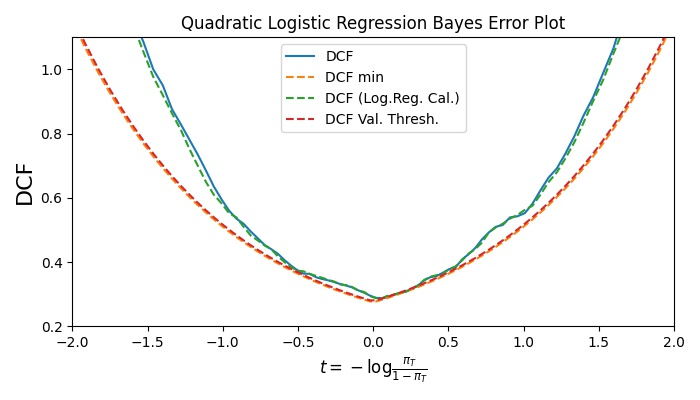
\includegraphics[width=\linewidth]{logregquadBEP.jpg}}
    \caption{Quadratic LR BEP}
    \label{fig:quadlogregbep}
\end{figure}

\begin{figure}[H] 
    {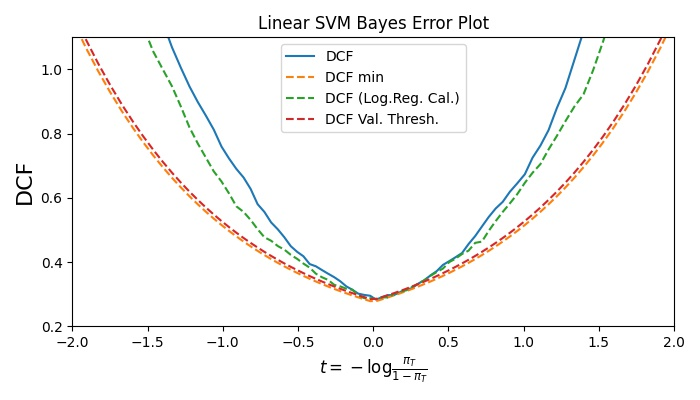
\includegraphics[width=\linewidth]{linsvmBEP.jpg}}
    \caption{Linear SVM BEP}
    \label{fig:linsvmbep}
\end{figure}

\begin{figure}[H] 
    {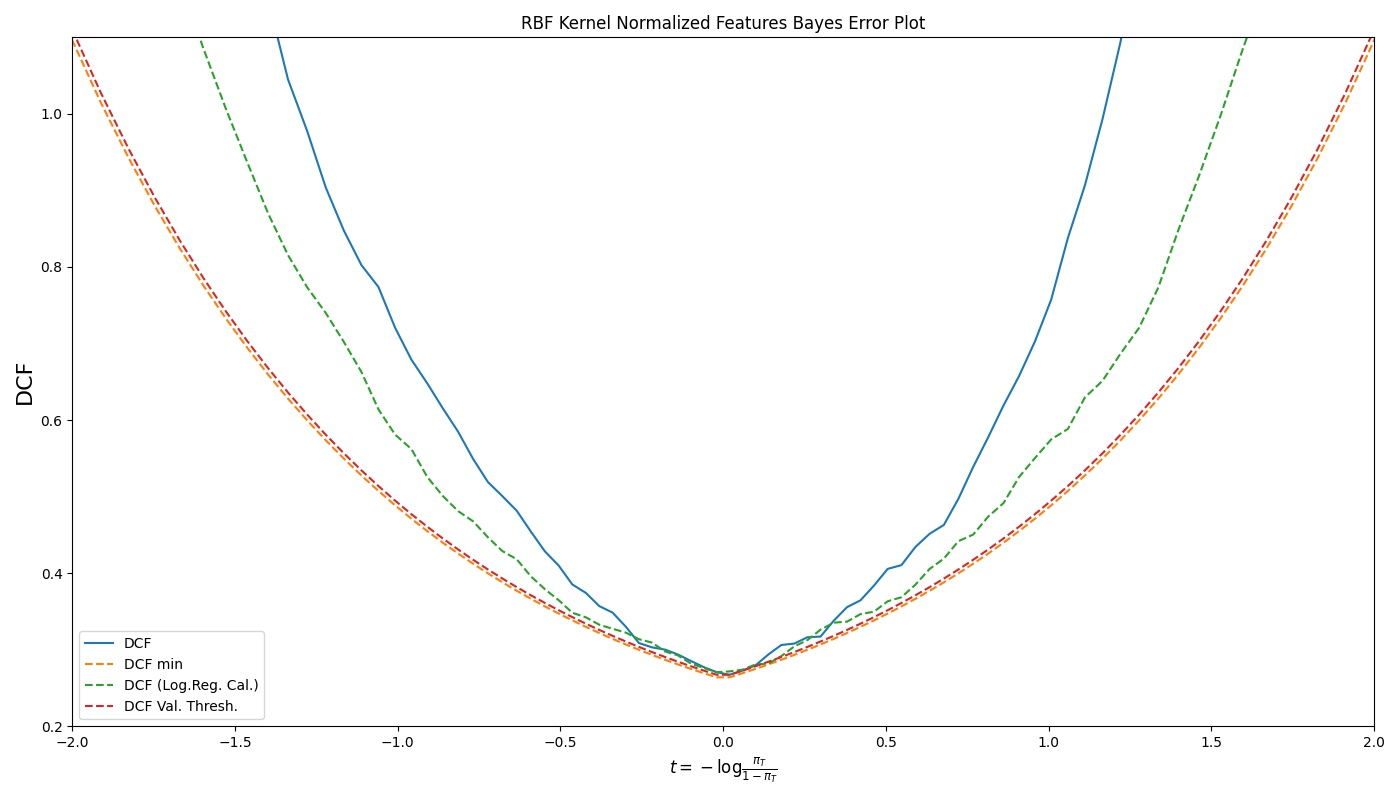
\includegraphics[width=\linewidth]{RBFNormalizedBEP.jpg}}
    \caption{RBF Kernel BEP}
    \label{fig:rbfkernelbep}
\end{figure}

\begin{table*}[t] 
    \centering
    \begin{tabular}{||c|c|c|c|c|c|c||}
        \hline 
        Model & Calibration & Features & PCA & Hyper-Parameters & DCF & DCF$_{min}$ \\
        \hline
        Linear LogReg & No & Normalized & 9 & $\lambda = 0.01$ & 0.303 & 0.299 \\
        Quadratic LogReg & Yes & Normalized & 10 & $\lambda = 0.001$ & {\bf 0.285} & 0.274 \\
        Linear SVM & Yes & Normalized & 9 & K = 10, C = 0.1 & {\bf 0.276} & 0.270 \\
        MVG Tied Cov. & No & Normalized & 5 & - & 0.390 & 0.331 \\
        GMM & No & Raw & No & $N_{Comp} = 2 $ & 0.327 & 0.294 \\ 
        RBF Kernel & No & Normalized & 10 & $\gamma = 0.05, C = 1.5, \xi = 0.1$  & {\bf 0.271} & 0.261 \\
        \hline
    \end{tabular}
    \caption{Final Parameters and Results on Test Set}
\end{table*}

Recalibrating scores helps most of the time, but our best option is
using a threshold computed from the validatiion scores.

Note that we trained our model and selected the hyper-parameters for a balanced case:
normally we should also tune them considering the target application,
meaning we should have trained the models differently for different applications.
In that case, score recalibrating may have been less important.


\end{document}